\chapter{温度与温度计}\label{ch:g3:temperature-thermometers}

两个冬天前，三碗水骗过了你的双手：同一碗水，
一只手觉得暖，另一只手却觉得凉。当时我们就许诺，
总有一天要用一种仪器来平息这类争论。它就是
\omterm{def:g3:temperature-thermometers:temperature}{温度计}——这个小小的玻璃“裁判”，
能把冷热变成一个数字。

\section{为什么触觉并不可靠}

\begin{example}[不公正的“裁判”]\label{ex:g3:temperature-thermometers:unfair}
触觉在每个季节都会“误判”：同样处于阴凉处，金属滑梯
摸上去比木质长椅更冷；温水对冷手是暖的，对暖手却是凉的；
玩过雪橇后，冷飕飕的走廊摸上去反而暖和。
要诚实地比较冷热——跨房间、跨日子、跨人——
我们就需要一个始终不改主意的裁判：
仪器。
\end{example}

\section{温度计及其刻度}

\begin{definition}[温度]\label{def:g3:temperature-thermometers:temperature}
物体的\emph{温度}\index{温度}，是一个说明它
究竟有多热或多冷的数。数越大，物体越热；数越小，物体越冷。
温度以\emph{摄氏度}\index{摄氏度}为\omterm{def:g2:measuring-length:measure}{单位}，
写作\unit{\celsius}，
用\emph{温度计}\index{温度计}\omterm{def:g2:measuring-length:measure}{测量}。
\end{definition}

\begin{proposition}[水的两个“里程碑”]\label{prop:g3:temperature-thermometers:milestones}
摄氏温标以水的两次重大状态变化为依据：
\begin{enumerate}
  \item 在 \qty{0}{\celsius} 时，水\omterm{def:g2:ice-water-steam:meltfreeze}{凝固}成冰（冰也会\omterm{def:g2:ice-water-steam:meltfreeze}{熔化}）；
  \item 在 \qty{100}{\celsius} 时，水沸腾成水蒸气。
\end{enumerate}
两个“里程碑”之间，温标被均分为 $100$ 等份——
从冰到水蒸气，就是一级级更小的台阶。
\end{proposition}

\begin{omfigure}
\begin{tikzpicture}[scale=0.85]
  \draw[thick] (0.5,0) rectangle (1.1,6.0);
  \draw[thick] (0.8,0) circle (0.42);
  \fill[omThm, opacity=0.7] (0.8,0) circle (0.34);
  % scale: 0 C at y=0.6, one unit of height per 20 C -> 25 C at y=1.85
  \fill[omThm, opacity=0.7] (0.62,0.05) rectangle (0.98,1.85);
  \foreach \y/\t in {0.6/0, 1.6/20, 2.6/40, 3.6/60, 4.6/80, 5.6/100} {
    \draw (1.1,\y) -- (1.35,\y);
    \node[right, font=\footnotesize] at (1.4,\y) {$\t$};
  }
  \foreach \y in {1.1, 2.1, 3.1, 4.1, 5.1} {
    \draw (1.1,\y) -- (1.25,\y);
  }
  \node[right, font=\small, omDef] at (2.6,0.6)
    {\qty{0}{\celsius}：水凝固};
  \node[right, font=\small] at (2.6,1.85)
    {\qty{25}{\celsius}：此时的读数};
  \node[right, font=\small, omThm] at (2.6,5.6)
    {\qty{100}{\celsius}：水沸腾};
  \draw[-Stealth, omExo] (2.5,1.85) -- (1.05,1.85);
\end{tikzpicture}

{\small \omterm{def:g3:temperature-thermometers:temperature}{温度计}：受热时红色\omterm{def:g3:solids-liquids-gases:liquid}{液体}上升。此时液面指在
刻度 $25$ 处，\omterm{def:g3:temperature-thermometers:temperature}{温度}为 \qty{25}{\celsius}。}
\end{omfigure}

\begin{example}[玻璃“裁判”的工作原理]\label{ex:g3:temperature-thermometers:works}
\omterm{def:g3:temperature-thermometers:temperature}{温度计}细细的管子里，封闭着一段有颜色的\omterm{def:g3:solids-liquids-gases:liquid}{液体}。
受热时，\omterm{def:g3:solids-liquids-gases:liquid}{液体}只会微微膨胀——但管子很细，
微小的膨胀也会让液柱明显上升；遇冷则收缩，液柱随之下降。
\omterm{def:g3:solids-liquids-gases:liquid}{液体}不会像手一样被骗：同样的热度，
今天、明天，对每个人而言，它膨胀的程度都一样。
\end{example}

\begin{omfigure}
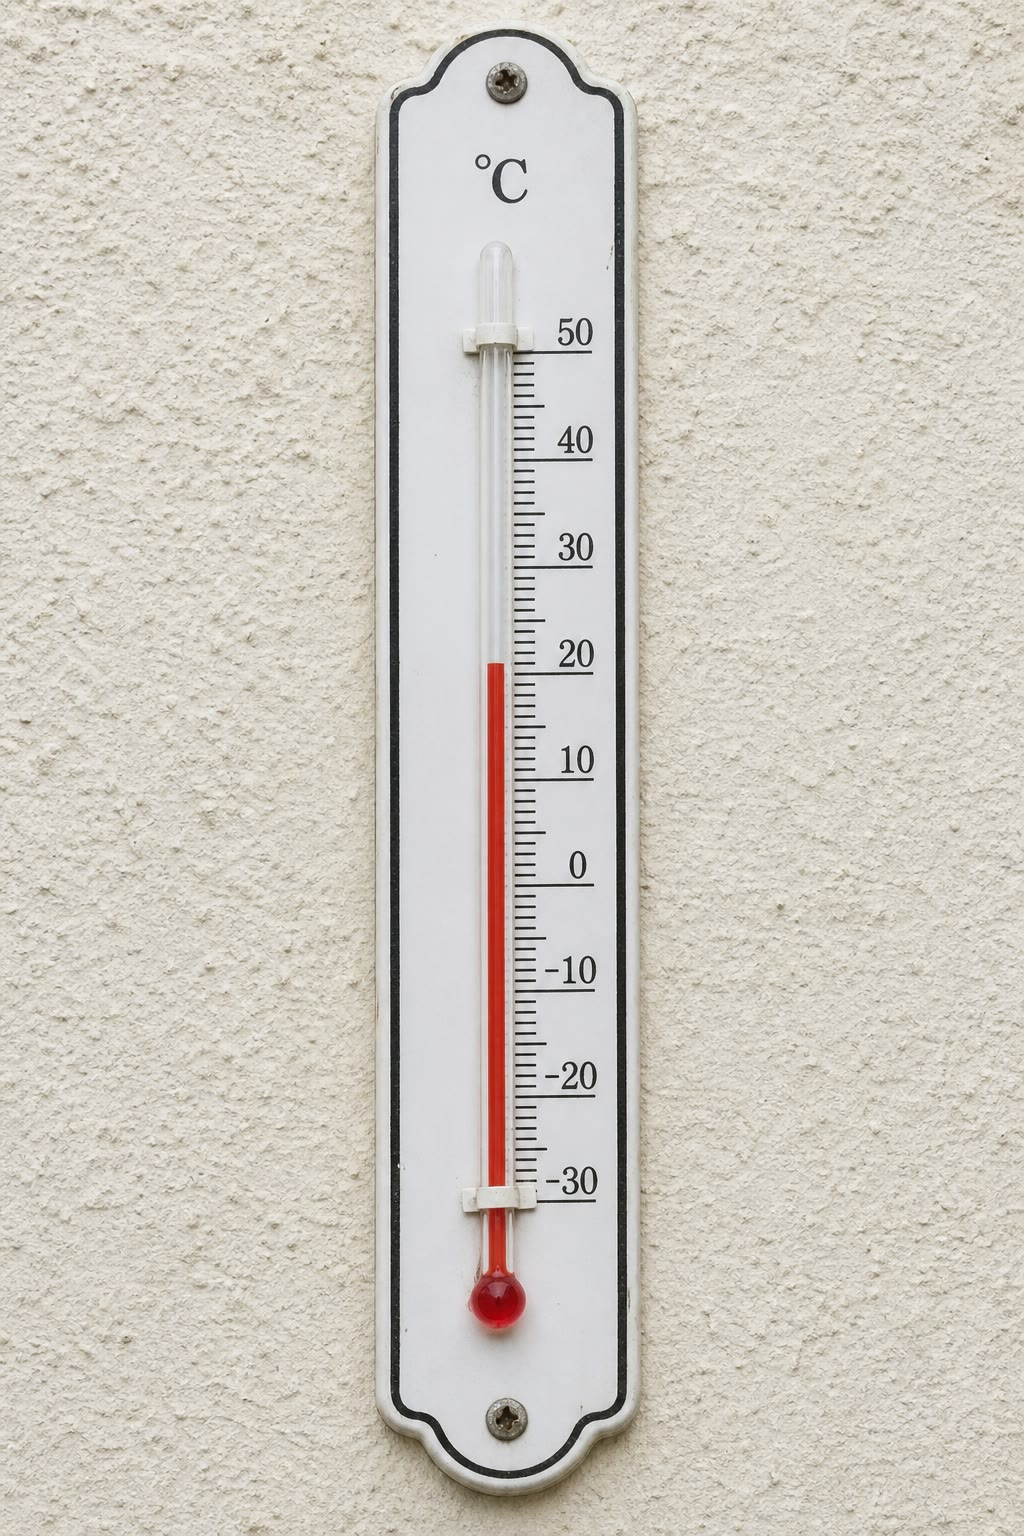
\includegraphics[width=0.3\linewidth]{images/book1/ai/g3-thermometer-outdoor.jpg}

{\small 墙上挂着的一支真实\omterm{def:g3:temperature-thermometers:temperature}{温度计}：红色液柱沿刻度上升，读取刻度的人都会得到同一个数字。}
\end{omfigure}

\section{读取温度计}

\begin{method}[读取温度计]\label{met:g3:temperature-thermometers:read}
\begin{enumerate}
  \item 把\omterm{def:g3:temperature-thermometers:temperature}{温度计}放到需要测温的地方——
        水中、户外阴凉处或舌下；
  \item \emph{等待}——\omterm{def:g3:solids-liquids-gases:liquid}{液体}需要时间完成上升
        或\omterm{def:g1:floating-and-sinking:words}{下沉}，直到液柱不再移动为止；
  \item 让眼睛与液柱顶端保持水平；
  \item 读出液柱顶端对准的刻度数字，
        并连同\omterm{def:g2:measuring-length:measure}{单位}写下：\qty{18}{\celsius}。
\end{enumerate}
读数过早，或从斜侧方向看，都会得出错误的数字——
裁判是诚实的，但读数要讲究方法。
\end{method}

\begin{example}[生活中的温度]\label{ex:g3:temperature-thermometers:livedby}
有些数值值得牢记：舒适的房间约为
\qty{20}{\celsius}；人的体温始终保持在约
\qty{37}{\celsius}，无论夏天还是冬天（明显高于此即为发烧，
医生的\omterm{def:g3:temperature-thermometers:temperature}{温度计}能说明这一点）；冰箱大约保持在 \qty{4}{\celsius}；
炎热的夏日可达 \qty{30}{\celsius}；
洗澡水\omterm{def:g3:temperature-thermometers:temperature}{温度}适宜时约为 \qty{35}{\celsius}。
\end{example}

\begin{omfigure}
\begin{tikzpicture}[scale=0.85]
  \foreach \x/\h/\t/\name in {0/1.1/4/冰箱,
      3.0/2.1/20/舒适的房间, 6.0/3.0/37/你的身体,
      9.0/2.6/30/夏日} {
    \draw[thick] (\x,0) rectangle ++(0.42,3.6);
    \fill[omThm, opacity=0.7] (\x+0.08,0.05) rectangle ++(0.26,\h);
    \node[above, font=\footnotesize] at (\x+0.21,3.65)
      {$\t$\,\unit{\celsius}};
    \node[below, font=\small, align=center] at (\x+0.21,-0.2) {\name};
  }
\end{tikzpicture}

{\small 四种常见\omterm{def:g3:temperature-thermometers:temperature}{温度}：液柱越高，
东西就越热。}
\end{omfigure}

\section{零下温度}

\begin{example}[冬季的数字]\label{ex:g3:temperature-thermometers:belowzero}
在寒冷的早晨，液柱会\omterm{def:g1:floating-and-sinking:words}{下沉}到 $0$ 刻度\emph{以下}。
那里的刻度继续往下排，读数时要加一个“负”字：
零下一格是\emph{负一}度，零下五格
是\emph{负五}度，写作 \qty{-5}{\celsius}。
负数比零度更冷，数字越小，
冻得越厉害：$-10$ 的早晨比 $-2$ 的更冷。
天气预报每个冬天的晚上都会报出这些数字。
\end{example}

\begin{remark}[零不是“没有”]\label{rem:g3:temperature-thermometers:zero}
在这个刻度上，$0$ 并不表示“没有\omterm{def:g3:temperature-thermometers:temperature}{温度}”——它只是
水结冰的那一格，像一块路标式的里程碑。天气
可能比这个刻度更暖，也可能更冷；\omterm{def:g3:temperature-thermometers:temperature}{温度计}
只告诉你在哪一侧、相差几格。（零下
的数字有一套自己的算法——你的数学
课会在以后的年级中正式学习。）
\end{remark}

\section{练习}

\begin{exercise}[$\star$]\label{exo:g3:temperature-thermometers:1}
为什么\omterm{def:g3:temperature-thermometers:temperature}{温度计}比你的手更能公正地判断冷热？
说出前面章节中一个手曾被欺骗的例子。
\end{exercise}

\begin{exercise}[$\star$]\label{exo:g3:temperature-thermometers:2}
水在什么\omterm{def:g3:temperature-thermometers:temperature}{温度}下结冰？在什么\omterm{def:g3:temperature-thermometers:temperature}{温度}下沸腾？
这两个数字用的是哪种\omterm{def:g2:measuring-length:measure}{单位}？
\end{exercise}

\begin{exercise}[$\star$]\label{exo:g3:temperature-thermometers:3}
\omterm{def:g3:temperature-thermometers:temperature}{温度计}受热时，细管里的\omterm{def:g3:solids-liquids-gases:liquid}{液体}会怎样变化？
冷却时呢？为什么这么小的变化
也能看得如此清楚？
\end{exercise}

\begin{exercise}[$\star$]\label{exo:g3:temperature-thermometers:4}
列出 \cref{met:g3:temperature-thermometers:read}
中提醒的读取\omterm{def:g3:temperature-thermometers:temperature}{温度计}时要避免的两个错误。
\end{exercise}

\begin{exercise}[$\star$]\label{exo:g3:temperature-thermometers:5}
将每样东西与其可能的\omterm{def:g3:temperature-thermometers:temperature}{温度}配对——
\qty{4}{\celsius}, \qty{20}{\celsius}, \qty{37}{\celsius},
\qty{100}{\celsius}：沸水；\ 舒适的客厅；\ 
冰箱内部；\ 你自己的身体。
\end{exercise}

\begin{exercise}[$\star$]\label{exo:g3:temperature-thermometers:6}
洗澡水的\omterm{def:g3:temperature-thermometers:temperature}{温度计}显示 \qty{35}{\celsius}；灶台上的锅
显示 \qty{100}{\celsius}。哪一个更热？这口锅
能否安全触摸？锅比洗澡水热多少度？
\end{exercise}

\begin{exercise}[$\star$]\label{exo:g3:temperature-thermometers:7}
冬季的\omterm{def:g3:temperature-thermometers:temperature}{温度计}显示液柱在零下 $3$ 格处。
这个\omterm{def:g3:temperature-thermometers:temperature}{温度}应当怎样读、怎样写？它比
\qty{-8}{\celsius} 更冷还是更暖？
\end{exercise}

\begin{exercise}[$\star$]\label{exo:g3:temperature-thermometers:8}
昨天花园里的\omterm{def:g3:temperature-thermometers:temperature}{温度计}早餐时显示 \qty{6}{\celsius}，
午饭时显示 \qty{14}{\celsius}。上午
升温了多少度？
\end{exercise}

\begin{exercise}[$\star$]\label{exo:g3:temperature-thermometers:9}
人行道上的积水一夜之间结成了冰。不用\omterm{def:g3:temperature-thermometers:temperature}{温度计}，你能
说出夜间\omterm{def:g3:temperature-thermometers:temperature}{温度}的什么信息？你用的是
哪一个刻度作为依据？
\end{exercise}

\begin{exercise}[$\star\star$]\label{exo:g3:temperature-thermometers:10}
爱玛刚玩完雪橇，就跑进门厅大喊：“这里
热得像在沸腾！”门厅的\omterm{def:g3:temperature-thermometers:temperature}{温度计}显示
\qty{16}{\celsius}。门厅热吗？爱玛为什么会有这种感觉——
以及家人应当相信哪一个判断者？
\end{exercise}

\begin{exercise}[$\star\star$]\label{exo:g3:temperature-thermometers:11}
一位厨师想知道，汤在大火翻滚时，
沸腾的时间越长，汤是否越热。她\omterm{def:g2:measuring-length:measure}{测量}：沸腾一分钟后，
\qty{100}{\celsius}；沸腾十分钟后，仍是 \qty{100}{\celsius}。
\omterm{def:g3:temperature-thermometers:temperature}{温度计}告诉她关于沸水的什么道理——
以及水的那些关键刻度？
\end{exercise}
